\chapter{Perbaikan Citra}
\section{Pendahuluan}

Perbaikan citra dilakukan dengan cara menghilangkan/mengurangi degradasi citra yang dapat disebabkan karena \textit{noise} atau \textit{blurring}. Degradasi sebuah citra digital dapat dimodelkan dengan persamaan (\ref{eq:degradeModel})\cite{Gonzalez}.

\begin{equation}
g(x,y)=\left(f(x,y)*h(x,y)\right)+n(x,y)
\label{eq:degradeModel}
\end{equation}
 
 Dari persamaan (\ref{eq:degradeModel}), diketahui
 \begin{itemize}
   \item $g(x,y)$ adalah citra terdegradasi
   \item $f(x,y)$ adalah citra asli
   \item $h(x,y)$ adalah filter spasial
   \item $n(x,y)$ adalah \textit{noise}
 \end{itemize}
 Dengan demikian, secara teoritis, citra asli dapat kembali diperoleh dengan menggunakan persamaan (\ref{eq:restore}). Tentu dengan mengetahui fungsi \textit{noise} yang menyebabkan citra terdegradasi.
 
 \begin{equation}
   f(x,y)=\frac{g(x,y)-n(x,y)}{h(x,y)}
   \label{eq:restore}
 \end{equation}
 
 \section{\texttt{random\_noise}}
 Pustaka \texttt{scikit-image} menyediakan fungsi degradasi citra dengan nama \texttt{random\_noise} yang diletakkan di bawah sub modul \texttt{util}. Fungsi tersebut memfasilitasi pemberian beberapa jenis \textit{noise} berikut karakteristiknya masing-masing. Berikut adalah beberapa contoh pemberian \textit{noise}. 
 
 Fungsi \texttt{random\_noise} menerima argumen berikut ini.
 \begin{enumerate}
   \item \texttt{image} adalah citra yang akan diberi \textit{noise}, fungsi akan secara otomatis melakukan normalisasi nilai intensitas citra pada rentang \texttt{0} s/d \texttt{1}.
   \item \texttt{mode} adalah jenis \textit{noise} yang dapat diberikan dalam tipe data \texttt{str}. Jenis \textit{noise} tersebut adalah
   \begin{itemize}
     \item 'gaussian' tambahan \textit{noise} yang memenuhi distribusi Gaussian
     \item 'localvar' tambahan \textit{noise} yang memenuhi distribusi Gaussian dengan tambahan informasi \textit{local variance} pada setiap titik citra. Jika argumen \texttt{mode} bernilai 'localvar', argumen \texttt{local\_vars} harus diberikan 
     \item 'poisson' tambahan \textit{noise} yang memenuhi distribusi Poisson
     \item 'salt' tambahan \textit{noise} yang mengubah titik piksel yang dipilih secara acak dengan nilai \texttt{1}
     \item 'pepper' tambahan \textit{noise} yang merupakan kebalikan dari 'salt'. \textit{Noise} 'pepper' mengubah titik piksel yang dipilih secara acak dengan nilai \texttt{1} (untuk jenis \textit{unsigned}) atau \texttt{-1} (untuk jenis \textit{signed})
     \item 's\&p' adalah tambahan \textit{noise} yang merupakan gabungan jenis 'salt' dan 'pepper'
     \item 'speckle' adalah tambahan \textit{noise} yang mengubah nilai intensitas citra pada setiap piksel menjadi $x+(n*x)$, dengan $x$ adalah intensitas citra asli dan $n$ adalah fungsi \textit{uniform noise} dengan tambahan argumen \texttt{mean} (rerata) dan \texttt{var} (varians) 
   \end{itemize}
   \item \texttt{seed} bertipe \texttt{int} dan bersifat opsional. Tetapi, jika nilai argumen diberikan, nilai tersebut akan digunakan untuk menghasilkan nilai acak untuk membangkitkan \textit{noise}
   \item \texttt{clip} bertipe \text{bool} dan bersifat opsional. Jika tidak diberikan, maka fungsi \texttt{random\_noise} akan memberikan nilai \texttt{True} pada argumen ini. Dampaknya, hasil pemberian \textit{noise} dari jenis 'speckle', 'poisson' dan 'gaussian' membuat citra tetap memiliki rentang nilai intensitas [-1,1] (\textit{unsigned}). Sebaliknya, jika secara aktif diberikan nilai \texttt{False}, citra hasil pemberian \textit{noise} dapat memiliki nilai intensitas di luar rentang normalnya
   \item \texttt{mean} adalah nilai rerata dari distribusi \textit{noise} 'gaussian' dan 'speckle'. Argumen ini bertipe \texttt{float} dan bersifat opsional. Jika tidak diberikan, fungsi \texttt{random\_noise} akan memberikan nilai \texttt{0} untuk argumen ini.
   \item \texttt{var} adalah nilai varians untuk distribusi \textit{noise} 'gaussian' dan 'speckle'. Argumen ini menerima nilai \texttt{float} dan bersifat opsional. Jika tidak diberikan, fungsi \texttt{random\_noise} akan memberikan nilai \texttt{0.01}
   \item \texttt{local\_vars} adalah argumen yang diperlukan ketike pengguna memberikan \textit{noise} dengan \texttt{mode} 'localvar'
   \item \texttt{amount} adalah argumen yang digunakan untuk menentukan proporsi jumlah piksel yang akan dikonversi nilai internsitasnya ketika \texttt{mode} 'salt', 'pepper' dan 's\&p' digunakan.
   \item \texttt{salt\_vs\_pepper} adalah argumen yang digunakan untuk menentukan proporsi jumlah piksel yang nilai intensitasnya akan dikonversi menjadi \texttt{1} ('salt') dan \texttt{0}/\texttt{-1} ('pepper'). Argumen ini diberikan ketika \texttt{mode} bernilai 's\&p'
 \end{enumerate}
 
\figurename~\ref{fig:addNoise} menunjukkan perbandingan citra asli dan citra dengan penambahan \textit{noise} dari fungsi Gaussian.
 
\begin{figure}[h!]
\begin{center}
\subfigure[]{\label{fig:asli}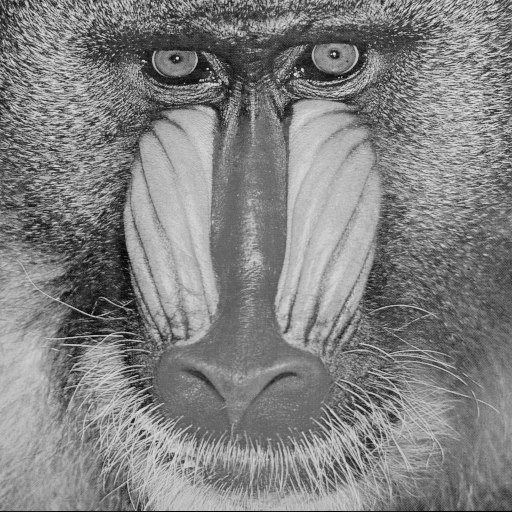
\includegraphics[scale=.35]{pics/baboonGS.png}}
\subfigure[]{\label{fig:nois}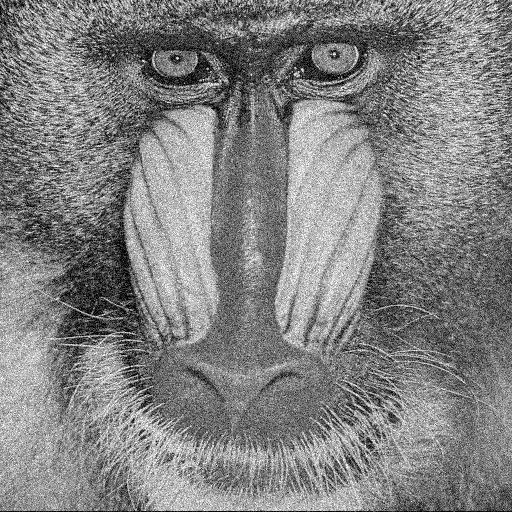
\includegraphics[scale=.35]{pics/baboonNoise.png}}
\caption{Perbandingan (a). citra asli, (b). citra dengan penambahan \textit{noise} Gaussian dengan nilai \texttt{mean=0} dan \texttt{var=0.01}}
\label{fig:addNoise}
\end{center}
\end{figure}
